\section{Введение}

В работе приводится пример системы двух дифференциальных уравнений, у которой минимальный траекторный аттрактор существует и состоит из функций, не являющихся решением этой системы. В частности, это дает существование глобального аттрактора этой системы. Конечно, в этом случае глобальный аттрактор понимается в смысле глобального аттрактора траекторных пространств (см. \cite{Chepyzhov}-\cite{umn}). То есть мы рассматриваем ситуацию, когда динамика системы описывается с помощью траекторных пространств и в этом случае глобальный аттрактор системы является сечением соответствующего минимального траекторного аттрактора. Однако, в силу факта существования и единственности решений рассматриваемой системы, ее динамику можно описать и с помощью полугруппы, т.е. динамической системы. Однако понятие глобального аттрактора динамической системы отличается от понятия глобального аттрактора траекторного пространства условием притягивания. Отметим, что для рассматриваемой системы, глобального аттрактора в смысле динамической системы не существует.

\par\medskip
%\section{}
\noindent \textbf{2.} Рассмотрим разбиение  $\mathbb{R}^2$ на пять непересекающихся связных множеств следующим образом:
$$
	A_0 = \{ (x_1, x_2) \mid 0 < x_1 < 1, 0 < x_2 < 1\},
$$
$$
	A_1 = \{ (x_1, x_2) \mid x_1 < 1, x_2 \leq 0  \}, \quad
	A_2 = \{ (x_1, x_2) \mid x_1 \geq 1, x_2 < 1  \}
$$
$$
	A_3 = \{ (x_1, x_2) \mid x_1 > 0, x_2 \geq 1  \}, \quad
	A_4 = \{ (x_1, x_2) \mid x_1 \leq 0, x_2 > 0  \}
$$
и отметим точки
$\alpha_1=(1, 0)$,
$\alpha_2=(1, 1)$,
$\alpha_3=(0, 1)$ и
$\alpha_4=\alpha_0=(0, 0)$
(последнее двойное обозначение используется для удобства работы с индексами).
Разбиение плоскости показано на рис. \ref{fig:somelabel}.

\begin{figure}[h]
	\centering
	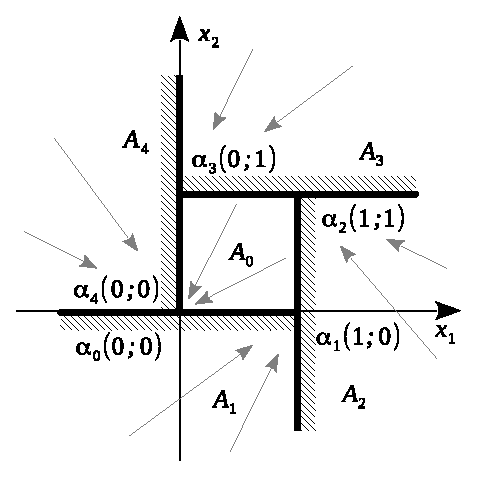
\includegraphics[width=0.4\linewidth]{quad3.eps}
	\caption{Разбиение плоскости, отмеченные точки и направления сдвигов}
	\label{fig:somelabel}
	%\vspace{2cm}
\end{figure}

Сразу заметим, что $\alpha_i \in \overline{A_i}$, $i=0,...,4$ и
$\alpha_i \in A_{i+1}$, $i=0,...,3$ (тогда как $\alpha_4 = \alpha_0 \in A_{1}$).

Таким образом, координатная плоскость оказалась разбита на четыре угла $A_1, \ldots, A_4$ и квадрат $A_0$.
Квадрат не включает свои границы; для каждого угла одна его сторона включается в угол,
а вторая сторона и вершина --- нет (они включаются в <<соседний>> угол).
Именно за счёт такого разбиения и достигается эффект примера.

В дальнейшем, в случае, когда нижних индексов два, первый нижний индекс
будет отвечать за номер области и обозначаться через $i$,
$i=0, ..., 4$, второй --- за номер координаты
(или соответствующего ей уравнения) и обозначаться $j$, $j=1, 2$.

Рассмотрим систему двух обыкновенных дифференциальных уравнений
\begin{equation}\label{difur_primer_R2}
	\frac{dx_j(t)}{dt} = -c_{ij} \cdot (x_j(t)-\alpha_{ij})^2, \quad j=1,2, \quad i=0,...,4, \quad t\geqslant 0,
\end{equation}
где, если
$
	(x_1, x_2) \in A_i,  \alpha_i = (\alpha_{i1},\alpha_{i2}),
$
$i=0,...,4$,
то
$
	c_{ij} = \operatorname{sgn}(x_j(0)-\alpha_{ij}),
$
в случае $x_j(0) - \alpha_{ij} \neq 0$,
и $c_{ij} = 0$ в противном случае.
Обратим внимание, что каждая координата точки траектории меняется независимо от другой,
и далее будет показано, что она стремится
к некоторому предельному значению.

Говоря подробнее,
$c_{ij}$ обращается в ноль только на границах углов $A_i$ и только для одной координаты на каждом луче,
образующем эти границы.
Например, на открытом луче, исходящем из точки $\alpha_2=(1, 1)$, направленном вниз и включенном в угол $A_2$, система (\ref{difur_primer_R2})
принимает вид:
\begin{equation*}
	\begin{cases}
		\dfrac{dx_1(t)}{dt} = 0, &\mbox{(т.к. $x_1(0) = 1 = \alpha_{21}$, имеем $c_{21} = 0$)},
	\\\\
		\dfrac{dx_2(t)}{dt} =  (x_2(t)-1)^2,  &\mbox{(т.к. $x_2(0) < 1 = \alpha_{22}$, имеем $c_{22} = -1$).}
	\end{cases}
\end{equation*}

Во внутренних точках угла $A_2$, т.е. не лежащих на этом луче, имеем:
$x_1(0) - \alpha_{21} = x_1(0) - 1 > 0$ и следовательно $c_{21} = 1$;
$x_2(0) - \alpha_{22} = x_2(0) - 1 < 0$ и следовательно $c_{22} = -1$.
Таким образом, во внутренности угла $A_2$ система (\ref{difur_primer_R2})
принимает вид:
\begin{equation*}
	\begin{cases}
		\dfrac{dx_1(t)}{dt} =  - (x_1(t)-1)^2,
	\\\\
		\dfrac{dx_2(t)}{dt} =  (x_2(t)-1)^2.
	\end{cases}
\end{equation*}

Вернёмся к общему виду системы (\ref{difur_primer_R2}).
Для $c_{ij} \neq 0$ решения системы (\ref{difur_primer_R2}) на $[0, \infty)$ имеют вид
\begin{equation}\label{primer_R2_x_j}
	x_j(t) = \frac{c_{ij}}{t+C_0}+\alpha_{ij}, \quad C_0 > 0,
\end{equation}
откуда
$
	x_j(t) \xrightarrow[t\to \infty ]{}{\alpha_{ij}},
$
при этом знак разности $x_j(t) - \alpha_{ij}$ не меняется (поскольку числитель дроби не зависит от $t$, а знаменатель всегда строго положителен).
Если же $c_{ij}=0$, то легко видеть, что $x_j(t) = x_j(0) = \alpha_{ij}$,
и формула (\ref{primer_R2_x_j}) также верна.

Выпишем теперь оператор сдвига.
Положим в (\ref{primer_R2_x_j}) $t=0$, получим
$
	x_j(0) = c_{ij}/{C_0}+\alpha_{ij}.
$

Выразив отсюда $C_0$, подставим его и $c_{ij}$ в (\ref{primer_R2_x_j}).
Таким образом, оператор сдвига по траекториям уравнения (\ref{difur_primer_R2}) имеет вид
\begin{equation}\label{primer_R2_oper_sdviga}
	(S_t(b_1,b_2))_j = \frac{b_{j}-\alpha_{ij}}{|b_{j}-\alpha_{ij}|t+1}+\alpha_{ij}, \quad j=1,2.
\end{equation}

Заметим, что числитель дроби не зависит от $t$, а знаменатель всегда строго положителен.
Следовательно, разность $(S_t(x_1(0), x_2(0)))_j - \alpha_{ij}$ сохраняет знак,
и траектория, начавшись в области $A_i$, никогда не перейдёт в другую область $A_{i'}$, $i \neq i'$.

Для $x_0 \in A_i$ имеем
\begin{equation}\label{primer_R2_stremlenie}
	S_t(x_0) \xrightarrow[t \to \infty]{} \alpha_{i},
\end{equation}
причём монотонно по $t$.
Действительно,
\begin{multline}\label{oper_sdviga_estimation}
	\|S_t(x_0) - \alpha_i\| \leq
	\sqrt{2} \max_{j=1,2} \left| \frac{x_{j}(0)-\alpha_{ij}}{|x_{j}(0)-\alpha_{ij}|t+1} + \alpha_{ij} - \alpha_{ij}  \right| =
	\sqrt{2} \max_{j=1,2} \left| \frac{x_{j}(0)-\alpha_{ij}}{|x_{j}(0)-\alpha_{ij}|t+1} \right| \leq
	\\ \leq
	\sqrt{2} \max_{j=1,2} \left| \frac{x_{j}(0)-\alpha_{ij}}{|x_{j}(0)-\alpha_{ij}|t} \right| =
	\sqrt{2} \max_{j=1,2} \left| \frac{1}{t} \right| =
	\frac{\sqrt{2}}{t} \xrightarrow[t \to \infty]{} 0.
\end{multline}

Заметим, что эта оценка не зависит от начального условия.
Более того, из того, что $\alpha_i \in A_{i+1}$, $i=0,...,3$,
следует, что $S_t(\alpha_i) \xrightarrow[t \to \infty]{} \alpha_{i+1}$,
т.~е. множество функций-констант
\begin{equation}\label{6}
	U = \{ u_i(t) \equiv \alpha_i \}_{i=0}^{3}
\end{equation}
не пересекается со множеством решений уравнения (\ref{difur_primer_R2}).

Покажем теперь, что $U$ --- траекторный аттрактор в смысле \cite{Vorotnikov2}-\cite{umn}.
Для этого напомним определение траекторного аттрактора и связанных с ним других абстрактных понятий. Пусть $E$, $E_0$ --- банаховы пространства, $E\subseteq E_0$ (вложение непрерывно) и $E$ --- рефлексивно. Символом $C(\mathbb{R}_+;E_0)$ обозначают пространство непрерывных функций, определенных на $\mathbb{R}_+=\{t\in\mathbb{R};\, t\geqslant 0\}$ и принимающих значение в $E_0$, символом $L_\infty(\mathbb{R}_+;E)$ обозначают пространство существенно ограниченных функций, определенных почти всюду на $\mathbb{R}_+$ и принимающих значение в $E$. Далее, непустое семейство функций $\mathcal{H}^+\subset C(\mathbb{R}_+;E_0) \cap L_\infty(\mathbb{R}_+;E)$ называется пространством траекторий, а его элементы --- траекториями. На пересечении $C(\mathbb{R}_+;E_0) \cap L_\infty(\mathbb{R}_+;E)$ рассматриваются операторы сдвигов $T(h)u(t)=u(t+h)$, $t,h\in\mathbb{R}_+$. Следующее важное понятие: непустое множество $P\subset C(\mathbb{R}_+;E_0) \cap L_\infty(\mathbb{R}_+;E)$ называется притягивающим (для $\mathcal{H}^+$), если для всякого множества $B\subset \mathcal{H}^+$, ограниченного в $L_\infty(\mathbb{R}_+;E)$ выполнено $\sup\limits_{u\in B}\inf\limits_{v\in P}\|T(h)u-v\|_{C(\mathbb{R}_+;E_0)}\to 0$ при $h\to\infty$. Наконец, непустое множество $U\subset C(\mathbb{R}_+;E_0) \cap L_\infty(\mathbb{R}_+;E)$ называется траекторным аттрактором пространства траекторий, если оно удовлетворяет следующим условиям: 1) множество $U$ компактно в $C(\mathbb{R}_+;E_0)$ и ограничено в $L_\infty(\mathbb{R}_+;E)$, 2) имеет место равенство $T(h)U=U$ для всех $h\geqslant 0$, 3) множество $U$ является притягивающим (для $\mathcal{H}^+$) (это определение содержится в \cite{Vorotnikov2}-\cite{umn}, оно отличается от соответствующего определения в \cite{Chepyzhov}-\cite{Sell} тем, что не предполагается включение $U\subset \mathcal{H}^+$). Траекторный аттрактор называется минимальным, если он содержится в любом другом траекторном аттракторе $\mathcal{H}^+$. Далее, множество $\mathcal{A}\subset E$ называется глобальным аттрактором (в $E_0$) пространства $\mathcal{H}^+$, если оно удовлетворяет следующим условиям: 1) множество $\mathcal{A}$ компактно в $E_0$ и ограничено в $E$, 2) для всякого ограниченного в $L_\infty(\mathbb{R}_+;E)$ множества $B\subset \mathcal{H}^+$ выполнено условие притягивания $\sup\limits_{u\in B}\inf\limits_{y\in \mathcal{A}}\|u(t)-y\|_{E_0}\to 0$ при $t\to\infty$, 3) множество $\mathcal{A}$ является наименьшим по включению, удовлетворяющим условиям 1) и 2). Ценность концепции минимального траекторного аттрактора заключается в том, что она позволяет решить проблему существования глобального аттрактора --- притягивающего множества в фазовом пространстве. Для множества $B\subset C(\mathbb{R}_+;E_0) \cap L_\infty(\mathbb{R}_+;E)$ определим сечение при некотором $t\geqslant 0$ формулой $B(t)=\{v(t);\,v\in B\}$. Имеет место следующий факт: пусть существует минимальный траекторный аттрактор $U$ пространства траекторий $\mathcal{H}^+$. Тогда существует глобальный аттрактор $\mathcal{A}$ пространства $\mathcal{H}^+$ и справедливо соотношение $\mathcal{A}=U(t)$, $t\geqslant 0$. В случае рассматриваемого в статье примера $E=E_0=\mathbb{R}^2$. Тогда для каждого $b=(x_1(0);x_2(0))$ определена функция $v_b\colon \mathbb{R}_+\to\mathbb{R}^2$ по формуле \eqref{primer_R2_oper_sdviga}. Определим пространство траекторий $\mathcal{H}^+$ как множество функций $\{v_b\}_{b\in \mathbb{R}^2}$. Тогда компактность и ограниченность множества из четырёх функций-констант в пространствах
$C(\mathbb{R}_+; \mathbb{R}^2)$ и $L_\infty(\mathbb{R}_+; \mathbb{R}^2)$ очевидна.
Очевидно и то, что $U$, определенное формулой \eqref{6}, трансляционно инвариантно.

Осталось показать, что $U$ есть притягивающее множество в $\mathcal{H}^+$ --- пространстве траекторий решений системы (\ref{difur_primer_R2}).
Действительно, пусть $M>0$ и $B\subset \mathcal{H}^+$ --- ограниченное в $L_\infty(\mathbb{R}_+; \mathbb{R}^2)$ множество.
Тогда 
\begin{multline*}
	\sup_{v\in B} \inf_{u\in U} \| T(t) v - u \|_{C([0,M];\mathbb{R}^2)} =
	\sup_{v\in B} \min_{i=0,..,3} \| T(t) v - u_i \|_{C([0,M];\mathbb{R}^2)} =
	\\ =
	\sup_{v\in B} \min_{i=0,..,3} \max_{s\in[0,M]} \| (T(t) v)(s) - u_i(s) \| =
	\sup_{v\in B} \min_{i=0,..,3} \max_{s\in[0,M]} \| (T(t) v)(s) - \alpha_i \| =
	\\ =
	\sup_{v\in B} \min_{i=0,..,3} \max_{s\in[t,t+M]} \| v(s) - \alpha_i \| \leq
	\frac{\sqrt{2}}{t} \xrightarrow[t\to + \infty]{} 0.
\end{multline*}
Таким образом, $U$ --- действительно траекторный аттрактор, пересечение которого с пространством решений системы (\ref{difur_primer_R2}) пусто.
Минимальный траекторный аттрактор содержится в любом траекторном аттракторе, в частности, в $U$,
следовательно, минимальный траекторный аттрактор в данном случае целиком лежит вне пространства траекторий пространства $\mathcal{H}^+$ (и он совпадает с $U$).

Таким образом, у системы (\ref{difur_primer_R2}) существует глобальный аттрактор в смысле траекторных пространств, являющийся сечением минимального траекторного аттрактора пространства $\mathcal{H}^+$.

%\section{}
\par\medskip

\noindent \textbf{3.} Покажем теперь, что глобального аттрактора полугруппы трансляций
в смысле динамической системы в данном примере не существует.
Предположим противное, т.е. что существует $P$ --- глобальный аттрактор полугруппы трансляций,
порождаемой оператором сдвига (\ref{primer_R2_oper_sdviga}).

Исходя из (\ref{primer_R2_oper_sdviga}) и (\ref{oper_sdviga_estimation}), легко заметить, что полугруппа, определяемая операторами сдвига (\ref{primer_R2_oper_sdviga}), ограничена.
Тогда, согласно Corollary 4.2.4 \cite{Zvyagin}, глобальный аттрактор полугруппы трансляций (динамической системы) совпадает с глобальным аттрактором в смысле траекторных пространств, который, в свою очередь, представляет собой сечение минимального траекторного аттрактора, т.е. множество
$$
	P = \{\alpha_i\}_{i=0}^3 = \{(0,0); (0,1); (1,0); (1,1)\}.
$$
Тогда по определению глобального аттрактора динамической системы должно выполняться равенство $S_t P = P$.
Однако, поскольку $\alpha_0 \in A_1$, то
$$
	(S_1(\alpha_0))_1 = (S_1(0,0))_1 =
	\frac{0-\alpha_{11}}{|0-\alpha_{11}|t+1}+\alpha_{11} =
	\frac{0-1}{|0-1|\cdot 1 +1}+1 = \frac{-1}{2} + 1 = \frac{1}{2}, 
$$
т.е. $S_1 \alpha_0 \notin P$, что противоречит определению глобального аттрактора динамической системы.

Полученное противоречие доказывает, что аттрактора полугруппы трансляций в данном случае не существует.


